\chapter{Approach}
\todo{Why are we using a data-driven / machine learning approach? Show that it is complicated to do it by hand. Also write why not to do auto-tuning.}

\begin{figure}
    \centering
    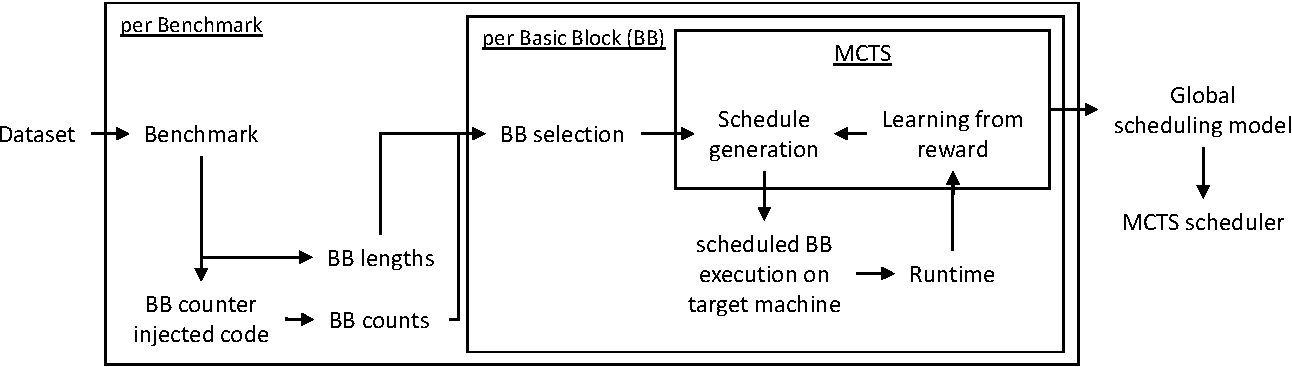
\includegraphics[width=\textwidth]{img/ppt/approach_overview-crop.pdf}
    \caption[Overview of the approach]{Overview of the overall approach. 
    The process covers the selection of basic blocks, the instruction schedule generation, the execution model, the learning process and the derivation of the final scheduler.}
    \label{fig:approach:overview}
\end{figure}
In the rest of this chapter, we will present the approach used for this thesis (compare~\cref{fig:approach:overview}).
We start with an overview of the benchmark programs we used~(\cref{sec:approach:dataset}).
Then we discuss the importance of basic blocks for instruction scheduling in general and our approach specifically~(\cref{sec:approach:basicblock}).
That is followed by explaining the \ac{mcts} approach~(\cref{subsec:approach:ml:mcts}).
Eventually, we introduce how we combine individual \ac{mcts} models into a global model~(\cref{subsec:approach:ml:global}) and derive an applicable scheduler~(\cref{sec:approach:ml-scheduler}).

\section{Dataset}
\label{sec:approach:dataset}
For our experiments, we use benchmarks from the LLVM project called LLVM Test Suite~\footnote{\url{https://llvm.org/docs/TestSuiteGuide.html}}.
The test suite contains benchmarks in the following categories
\begin{itemize}
    \item Single-Source --- built from a single C/C++ source file
    \item Multi-Source --- built from multiple C/C++ source files
    \item Micro-Benchmarks --- seperate functions, that are executed by google-benchmark
    \item Bitcode --- tests that are written in LLVM bitcode
    \item CTMark --- symbolic links to the other benchmarks to measure compilation performance
\end{itemize}
We select the 273 benchmarks from the Single-Source and Multi-Source categories for our experiments.
\todo{Add table?}
The benchmarks are all written in C or C++.
These categories contain benchmarks that are compiled from a single source file or multiple source files, respectively.
In addition, the test suite contains more benchmarks that are not relevant to our experiments or took too long to integrate.

\subsection{Modified build process}
\label{sec:approach:build_process}
The test suite comes with Makefile's and CMake configuration to automatically build all the benchmarks.
However, these are not sufficient for our approach.
We need a modified build process for all the benchmarks because we are manipulating it in several cases.
Furthermore, the compilation cannot be done with a single command because not all arguments of the separate compilation steps are available in the main compiler.
We execute the front-end, optimization, and back-end phase separately to have complete control over the build process.

We have to set some compiler arguments to make the LLVM compiler front-end eject LLVM \ac{ir} instead of compiling the program completely.
For C programs we use \lstinline{clang}~\footnote{\url{https://clang.llvm.org/}} and for C++ programs we use \lstinline{clang++}.
However, the compiler arguments are the same.
We pass the following arguments to the front-end:
\begin{itemize}
    \item \lstinline{-O0}: to prevent optimization in this first step
    \item \lstinline{-Xclang -disable-O0-optnone}: the \lstinline{-O0} flag alone also prevents optimization in further steps, which is not what we want
    \item \lstinline{-S -emit-llvm}: to emit LLVM \ac{ir} for further processing --- instead of compiling the program completely
\end{itemize}

The LLVM optimizer \lstinline{opt}~\footnote{\url{https://llvm.org/docs/CommandGuide/opt.html}} gives a choice to select one of the predefined optimization levels or select specific optimizer runs.
When we compile a benchmark for measuring the runtime, we only use the flag \lstinline{-O3} for optimizing the LLVM \ac{ir}.
The LLVM framework makes it easy to implement new optimizer passes.
We do this to count how often a basic block is executed (see \cref{sec:approach:basicblock:selection}) and measure a function's execution time (see \cref{sec:approach:datageneration:runtime:function}).

We manipulate the instruction scheduling by adjusting how we call the compiler back-end.
The LLVM static compiler implements two instruction schedulers before the register allocation and one after the register allocation.
The former inherit either from the C++ class \lstinline{SelectionDAG} or from \lstinline{MIScheduler}.
Which one will be executed by the compiler depends on the target architecture. 
It is also possible that the compiler executes both.

We manipulate the back-end by passing arguments to the LLVM static compiler \lstinline{llc}~\footnote{\url{https://llvm.org/docs/CommandGuide/llc.html}}.
This program represents the back-end phase and executes the instruction scheduling.
We use the following arguments for the back-end:
\begin{itemize}
    \item \lstinline{--pre-RA-sched=}: to select our new \lstinline{SelectionDAG} schedulers for the pre-register-allocation phase
    \item \lstinline{--misched-cutoff=0}: to disable the \lstinline{MIScheduler}
    \item \lstinline{--disable-post-ra}: to disable the post-register-allocation scheduler
\end{itemize}

We analyze the CMake configurations and extract required compiler arguments on a per benchmark level.
We categorize the extracted arguments into front-end, optimizer, and back-end phases.
Finally, we append them to the previously described arguments in the respective compilation phase.

We also analyze the test suite for execution arguments.
For example, some benchmarks read data from files or require arguments when calling them.
To execute them, we generate a shell script that calls the compiled benchmark with the required arguments.

\section{Basic Block --- scheduling unit}
\label{sec:approach:basicblock}
Even though there exists some research on instruction scheduling on more extensive units, most compilers schedule instructions on a per basic block level.
This is also true for the LLVM compiler framework.
The advantage of this is that the limited scope avoids complicated situations and thus simplifies the scheduling problem.
For Example, do not have to deal with jump instructions.

Consequently, we also choose the basic block as the unit for instruction scheduling.
That means that we execute our experiments on individual basic blocks and learn to schedule individual basic blocks.
Later, we combine the models to generalize the knowledge.
We describe this process in detail in \cref{sec:approach:ml}.

\subsection{Selection process}
\label{sec:approach:basicblock:selection}
Not all basic blocks provide an equal value to our experiments.
It also consumes too much time to work on all the basic blocks within the scope of this thesis (\eg compilation time, execution time, machine learning time).
Therefore, we sort our basic blocks by heuristics. 
From this list, we select as many as we need and can handle in our experiments.
We designed three heuristics which we will explain in the following paragraphs.
See \cref{tab:approach:bb_heuristics} for an example overview.

\begin{table}
    \centering
    \begin{tabular}{@{}llrrr@{}}
        \toprule
        Function & Basic Block & Length & \(\#\) Executions & Product \\
        \midrule
        kernel\_floyd\_warshall\_StrictFP & for.body6 & 23 & 536,870,912 & 12,348,030,976 \\
        kernel\_floyd\_warshall & for.body6 & 23 & 536,870,912 & 12,348,030,976 \\
        print\_element & entry & 25 & 1,048,576 & 26,214,400 \\
        kernel\_floyd\_warshall\_StrictFP & for.cond4.preheader & 17 & 1,048,576 & 17,825,792 \\
        \(\cdots\) & \(\cdots\) & \(\cdots\) & \(\cdots\) & \(\cdots\) \\
        xmalloc & entry & 8 & 2 & 16 \\
        main & entry & 11 & 1 & 11 \\
        \bottomrule
    \end{tabular}
    \caption[Basic block heuristics for the floyd-warshall benchmark]
    {
        The tables shows an excerpt of the basic block heuristics (see \cref{sec:approach:basicblock:selection}) for the floyd-warshall benchmark. 
        The basic blocks are sorted by the last heuristic, which is the product of the length and execution count. 
        From this list the table shows the top four and last two basic blocks in the benchmark.
    }
    \label{tab:approach:bb_heuristics}
\end{table}

\subsubsection{Longest basic blocks}
The number of instructions in a basic block correlates with the number of possible schedules.
Consequently, we can learn more from a basic block when there are more different scheduling situations available.
For example, we will see more scheduling situations in a basic block containing 20 instructions than in a basic block containing only three instructions.

We implemented a hook into the LLVM framework to count the number of instructions in a basic block.
This hook prints the number of instructions in each basic block during the compilation process.
From this output, we put together a list with all basic blocks and their lengths (see \cref{tab:approach:bb_heuristics}).

\subsubsection{Most executed basic blocks}
Some basic blocks are significantly more often executed than others.
For example, basic blocks in the bodies of loops run often.
A basic block in the error checking code of the beginning of a program might only execute once.
Often executed basic blocks influence the overall runtime a lot.
Hence, we are more interested in optimizing these.
See \cref{tab:approach:bb_heuristics} for an example.

We implemented a LLVM optimizer pass for injecting counters into a program.
Optimizer passes take LLVM \ac{ir} files as input and output the code in the same file format.
Our pass injects one global 64 bit counter variable for each basic block into the code.
Next, the pass adds instructions into the beginning of each basic block, which increase the corresponding counter by one.
At the end of the main function the pass adds a format string and injects a call to the \lstinline{printf} function to print all the counter values and corresponding basic block names.

The optimizer pass must be compiled with the LLVM framework.
We include the optimizer pass into our build process (see \cref{sec:approach:build_process}).
There, we add a call to the LLVM optimizer \lstinline{opt} with the argument \mbox{\lstinline{-passes=dyn-bb-count}}.
To actually get the counts, we build a benchmark with this optimizer pass and and execute it.
The benchmark will then print the counter values.

\subsubsection{Most executed and longest basic blocks}
The previous two heuristics are helpful on their own, but we are most interested in basic blocks that combine the two aspects.
For example, the most executed basic block can still come from a very simple loop with few instructions in the loop body.
We compute the product of the two heuristics to get a combined heuristic.

\section{Learning to schedule}
\label{sec:approach:ml}
\subsection{Local MCTS model}
\label{subsec:approach:ml:mcts}
\subsection{Global model}
\label{subsec:approach:ml:global}

\section{Data generation}
We cannot build our data-driven models (see \cref{sec:approach:ml}) directly from our dataset, described in \cref{sec:approach:dataset}.
Learning from this dataset requires some transformation from the code to a metric we are interested in.
Many metrics can be chosen for optimization \eg runtime, energy consumption, cache misses, processor stalls.
We focus on optimizing the instruction scheduling for fast runtimes.
To generate data for our MCTS approach we need a mapping from instruction schedules to runtimes.
Therefore, we compile the code with varying instruction schedules and execute it to measure its runtime.
We discuss various aspects of this in the remainder of this section.

\subsection{Runtime measurement unit}
It would be optimal to just measure the the scheduled instructions with perfect precision and reliability.
\subsubsection{Basic Block}
\begin{itemize}
    \item What: Measuring the basic block itself is complicated
    \item Why: we need very precise time measurements
    \item How: the typical length of a basic block ranges from a hand full of instructions to a few dozens
    \todo{Plot basic block length distribution}
\end{itemize}
\subsubsection{Function}
\label{sec:approach:datageneration:runtime:function}
A specific basic block of a function might be executed multiple times during function execution.
In this situation, this is relevant in to different aspects.

% \begin{itemize}
%     \item What: Advantage: BB is executed multiple times, so its runtime is easier to measure
%     \item Why: 
%     \item How: 
% \end{itemize}
We are more interested in speedups, rather than precise execution times.


\begin{itemize}
    \item What: Measure the function which contains the basic block is bad in general
    \item Why: Different paths could be taken throught the function, e.g. if-else, loops
    \item How: 
\end{itemize}
\begin{itemize}
    \item What: In this case it is okay
    \item Why: the benchmarks are deterministic, each path is taken the same number of times between executions
    \item How: 
\end{itemize}
\subsubsection{Program}
\begin{itemize}
    \item What: Measure the execution time of the whole program
    \item Why: Easy, but unreliable because of IO operations and other noise (e.g. OS), we are only interested in a small fraction of the code
    \item How: 
    \todo{Show visualization}
\end{itemize}

\subsection{Runtime measurement methods}
\todo{Could add little experiment where we compare hardware timers vs OS access}
\subsubsection{Profiling}
\begin{itemize}
    \item What: Profilers are a bad choice for measuring precise runtimes
    \item Why: They are just not designed for it, they serve other purposes.
        Profilers are making snapshots of the running system to measure performance. 
        There is no measurement from point A to point B which leads to inaccuracies
    \item How: Read e.g. the paper of gperf \cite{graham1982gprof}
\end{itemize}
\subsubsection{Operating system methods}
% In linux(C): clock_gettime().
% Windows: QueryPerformanceCounter().
% C++: std::high_resolution_clock().
These might return different clocks depending on the used hardware.
Returns the time from the hardware the OS runs on.
Has overhead but also handles problems.
Typically best for measurements in microseconds range and longer.
\subsubsection{Hardware performance counters}
Accessed by assembly instructions.
% x86: 'rdtsc' Saves current value into EDX:EAX registers
% ARM32: mrc p15m, 0, \%0, c15, c12, 1
% AARCH64: mrs \%0, PMCCNTR_EL0
% Aurora: fencei; smir \%0, \%usrcc
Measurements in CPU cycles.
Lowest overhead available.
Access might be protected (Linux module required).
\subsection{Basic block isolation}
\subsubsection{Basic block extraction}
How to get the assembly (compilation process).
Problems: function calls (remove), jumps(only in last instr, remove), load/access (memory access, readress to stack variable)
\todo{Create table with removed instructions}
\subsubsection{Isolated basic block execution}
From extracted basic block create inline assembly with stack variable. Now executable from C/C++.
Warmup 100 runs. Timings 1000 runs. 
\subsection{Computing rewards from runtimes}
There are some outliers in the runtimes. Sort runtimes, cutoff lower and upper 5\% of the runtimes to remove outliers and compute avg of the rest.
What could be reasons for outliers?
Show some distributions of measurements to justify why we are throwing away data.

\section{Application of the learned model}
\label{sec:approach:ml-scheduler}

% Probably wrong place here, but compare approach with auto-tuning approach.
% Why not use auto-tuning? Search space size, and lack of generalization could be a reason

% \section{Breaking down the problem (maybe just chapter introduction)}
% \begin{itemize}
%     \item Schedulers run on basic blocks -> Select the most executed (hottest) BB's
% \end{itemize}

% \section{Experimentation Pipeline}
% Explain and illustrate the pipeline incl. injection of timers and counters

% \section{Benchmarking}
% \begin{itemize}
%     \item Benchmarking methods: Instrumentation, sampling -> only instrumentation makes sense here. Justify this with instrumentation vs. sampling results (our timing vs. perf timing)
%     \item Where to inject timer in BB DAG
%     \begin{itemize}
%         \item We only want to measure optimized code, but not too kleinteilig because of lacking accuracy. Problematic code is IO code
%         \item Time whole function?
%         \item Time only relevant BB's with surrounding ones (e.g., loop headers) -> Where exactly place the the timer
%         \item Provide data and examples to demonstrate decision making
%     \end{itemize} 
% \end{itemize}
% \subsection{Implementation}
% Injection of the \lstinline[language=C++]{std::chrono::high_resolution_clock}

% \section{Training setup}
% Compile with default scheduler and measure its runtime.
% Compile with our scheduler, execute the program, measure the runtime and use it to train the agent.

% \section{MCTS}
% \subsection{Tree Modeling}
% We probably want to model the interdependence between instructions. 
% But depending on the benchmark programs, only a small fraction of possible edges between instructions are available.

% \eg When in the benchmark a MOV was scheduled and after that, there are only SUB and ADD.
% We cannot schedule another MOV even though that might be the optimal schedule.

% This problem must be addressed somehow.
% There are different possibilities:
% \begin{itemize}
%     \item Declare all the states with their possible successors to different states.
%     The problem with this approach is that the number of states gets very high and most states are visited rarely, possibly only in the given benchmark/basic-block.
%     \item Probablistic Policy like in RL. (Does that exist for MCTS?)
%     This might solve the problem with unavailable edges, but it does not help with learning at all because the agent would have to learn which instructions are available, too.
%     Which is not what we want.
% \end{itemize}